\chapter{Methodology}
\label{ch:method}

\begin{instructions}
About 4--5 pages. Built from the plan's Chapter 4 and corrected. The corpus is now 26 registered source files from at
least five species, not four oyster recordings. Native rates are kept rather than resampled to 1\,Hz. The judging
protocol (5.4) is new, and is what makes every result chapter's ``against blind human judgement'' meaningful. The
held-out section (5.6) records the planned protocol, what actually happened, and the exam as run.
\end{instructions}

This chapter describes the corpus, the preprocessing applied to it, how data are represented, how human judgements are collected, the controls that every reported result carries, and the held-out exam. Chapter~\ref{ch:pipeline} described the software; this chapter describes how it was used.

\section{Corpus}
\label{sec:corpus}

The recordings are long multi-electrode potential measurements from living fungal cultures. Most come from the Underground Brains research facility at UQ: \emph{Pleurotus ostreatus} (oyster) arrays of 16 electrodes with a shared ground, inside Faraday cages, plus later recordings of other species and setups. Three species come from Adamatzky's public four-species dataset \cite{adamatzky2021data}. Table~\ref{tab:corpus} lists every registered source file and its role in this thesis.

\begin{table}[htbp]
\caption{The corpus: 29 registered source files (20 active), with species, channels, native sampling rate, duration, units and role. Copies of one recording at another rate share a row. Hours are $n_\text{samples}/f_s$.}
\label{tab:corpus}
\footnotesize
\begin{tabularx}{\textwidth}{p{3.3cm} p{2.4cm} r r r l X}
\toprule
\textbf{Dataset} & \textbf{Species} & \textbf{Ch} & \textbf{$f_s$ (Hz)} & \textbf{Hours} & \textbf{Units} & \textbf{Role}\\
\midrule
M2\_aug\_concat\_fs1 & Oyster & 16 & 1 & 721 & V & Primary; RQ1--RQ3\\
M2\_concat\_fs1 & Lion's mane & 16 & 1 & 282.5 & V & Secondary; out-of-sample checks\\
M4\_aug\_concat\_fs1 & Oyster & 16 & 1 & 505 & -- & \textbf{Held out} (exam, Section~\ref{sec:holdout})\\
MJu26a (fs10; fs2 derived) & Lion's mane & 16 & 10, 2 & 636 & V & Round-B sweep at 2\,Hz (MJu26a\_fs2, 27 Oct)\\
L\_LM\_Jul\_26\_J (raw, fs2) & Lion's mane & 5 & 10, 2 & 636 & mV & Detector sweep; classifier. A copy of MJu26a CH10 and CH13--16 ($\times$1000 plus a constant offset; $r=1.00000$)\\
Mushroom\_260720 (rec.\ 385) & Lion's mane & 1 & 1 & 4 & V & Spiking-families pass; Library. A 4\,h excerpt of MJu26a CH14 (inactive)\\
LM\_fs2 & Lion's mane & 4 & 2 & 480 & V & Detector sweep; classifier\\
CO\_fs2 & Chocolate oyster & 4 & 2 & 480 & V & Detector sweep; classifier\\
SH, SO (fs2 derived) & ? & 4 & 10, 2 & 480 & V & Round-B sweep at 2\,Hz (27 Oct); 10\,Hz read from each file's time vector\\
F2B & ? & 5 & 10 & 144 & mV & Excluded: a subset of L\_LM\\
L\_R\_Aug\_26\_PD & ? & 13 & 10 & 107 & V & Excluded: humidity-actuator oscillation in the signal\\
Fig2A\_dt0p1 & Reishi & 5 & 10 & 0.3 & mV & Drop-motif study; Library (inactive)\\
M1, M100, M101\_t & Oyster & 13 & 10 & 302 & -- & Inactive; M101 has an environment log\\
\emph{S.\ commune} \cite{adamatzky2021data} & \emph{S.\ commune} & 7 & 1 & 73 & mV & Public; proposed second unseen test\\
\emph{C.\ militaris} & \emph{C.\ militaris} & 7 & 1 & 528 & mV & Public; complexity fingerprint\\
\emph{F.\ velutipes} & Enoki & 7 & 1 & 300 & mV & Public; complexity fingerprint\\
Dwij A--D & ? & 4 & 0.8 & 0.3--29.3 & mV & Registered\\
\bottomrule
\end{tabularx}
\end{table}

\begin{instructions}
Fill in the ``?'' species and the setup of each UQ dataset: LM, CO, SH, SO, F2B, L\_R and Dwij. Settings $\rightarrow$
Datasets declares five species today: oyster, lion's mane, split gill (\emph{S.\ commune}), \emph{Cordyceps} and enoki.
Reishi is undeclared (ledger A6). Check the units of the reishi file. The lion's mane excerpt
(recording 385) is in volts: it equals MJu26a CH14's 10-sample means (slope 1.0009, $r=0.9995$; ledger A17). State the
number of distinct physical recordings: the earlier ``about 18'' predates finding that L\_LM and recording 385 are
copies of MJu26a channels (ledger A16--A17). Facts from the \texttt{recordings} and \texttt{datasets} tables and
\src{docs/datasets/}.

Dataset decisions (26 Oct):
\begin{itemize}
  \item copies that are subsets of another recording, or the same recording at another rate, were deactivated, so
        that every active set is an independent recording;
  \item L\_R is excluded because the humidity actuator's PID controller in its tent oscillated, and that oscillation
        appears in the signal: ``motifs'' there could be humidity-driven changes in electrode conductivity;
  \item 10\,Hz sets are analysed as 2\,Hz derivations, to save compute.
\end{itemize}
Dataset work (27 Oct):
\begin{itemize}
  \item MJu26a, SH and SO were derived at 2\,Hz as CO\_fs2 and LM\_fs2 had been (non-overlapping means of five
        samples, nothing else changed) and registered. Their sweep bundle is
        \src{docs/thesis/hpc/rq4_newsets_20261027/}. The 10\,Hz originals stay active for now;
  \item L\_LM is MJu26a: its five channels are MJu26a CH10 and CH13--16, $\times$1000, plus a constant offset per
        channel (\src{docs/datasets/NEW_RAW_2026-10.md}). MJu26a\_fs2's sweep covers them again. Decide whether
        L\_LM raw is deactivated like the other copies.
\end{itemize}
Corrections to the plan:
\begin{itemize}
  \item the primary oyster recording is 721\,h, not over 1,000\,h. The ``about 1,000 hours'' is M2\_aug and M2\_concat,
        and M2\_concat is lion's mane (the researcher, 3 Nov), so it is not 1,000 hours of oyster. The oyster recordings
        are M2\_aug (721\,h) and the held-out M4 (505\,h); CO is chocolate oyster (480\,h at 2\,Hz);
  \item M2\_aug and M2\_concat are different data, not crops of each other (best $d/\sqrt{m}\approx0.79$);
  \item cross-species comparison is now possible in principle (Chapter~\ref{ch:events});
  \item the fourth Adamatzky species (\emph{Omphalotus nidiformis}) is in \src{DATA/raw} but not registered in the real
        database.
\end{itemize}
Consider a figure of one representative trace per species at a common scale.
\end{instructions}

\begin{figure}[htbp]
\centering
\figplaceholder{8cm}{Figure 5.1 (T1, bundle): the dataset gallery. One row per recording (M2\_aug, M2\_concat, M4,
MJu26a, LM, CO, SH, SO), each showing one channel over a day and a 30-minute zoom, in mV, coloured by species.}
\caption{What each recording in the corpus looks like.}
\label{fig:gallery}
\end{figure}

\section{Preprocessing}
\label{sec:preprocessing}

\begin{instructions}
Rewrite. The plan's resampling story (an 18\,Hz DAC with drifting $\Delta t$, resampled to 1\,Hz) is not what the
software does. As built:
\begin{itemize}
  \item each dataset keeps its native rate: 1\,Hz for the oyster arrays, 2 or 10\,Hz for others, 0.8\,Hz for Dwij.
        The rate is read from the file, inferred from the sample count, or stated by the researcher, and recorded in
        \texttt{fs\_source};
  \item uneven time axes are linearly interpolated onto a uniform grid (MJu26a: $\Delta t$ 0.124--2.83\,s onto 10\,Hz)
        by \src{scripts/derive_raw_mat.py};
  \item units are declared per dataset (V or mV), and every block that prints millivolts reads through
        \texttt{read\_as\_mv} (fixed 15 Oct, when the drop detector had assumed volts);
  \item gaps are skipped, NaN-aware, rather than refused (your decision, 14 Oct). Adamatzky's logger pauses were
        interpolated and every filled run is listed in the manifest;
  \item analysis is per channel. The ``concat'' files are 16-channel files of joined recording sessions, not one
        concatenated channel.
\end{itemize}
Artefacts: \texttt{artifact} is a human verdict. Cross-channel near-copies ($r\ge0.98$ where both are real events) are
machine-flagged into a suspected-artifact Review queue, and a human decides. Keep the plan's flagged-data figure as an
example of what is excluded.
\end{instructions}

\begin{figure}[htbp]
\centering
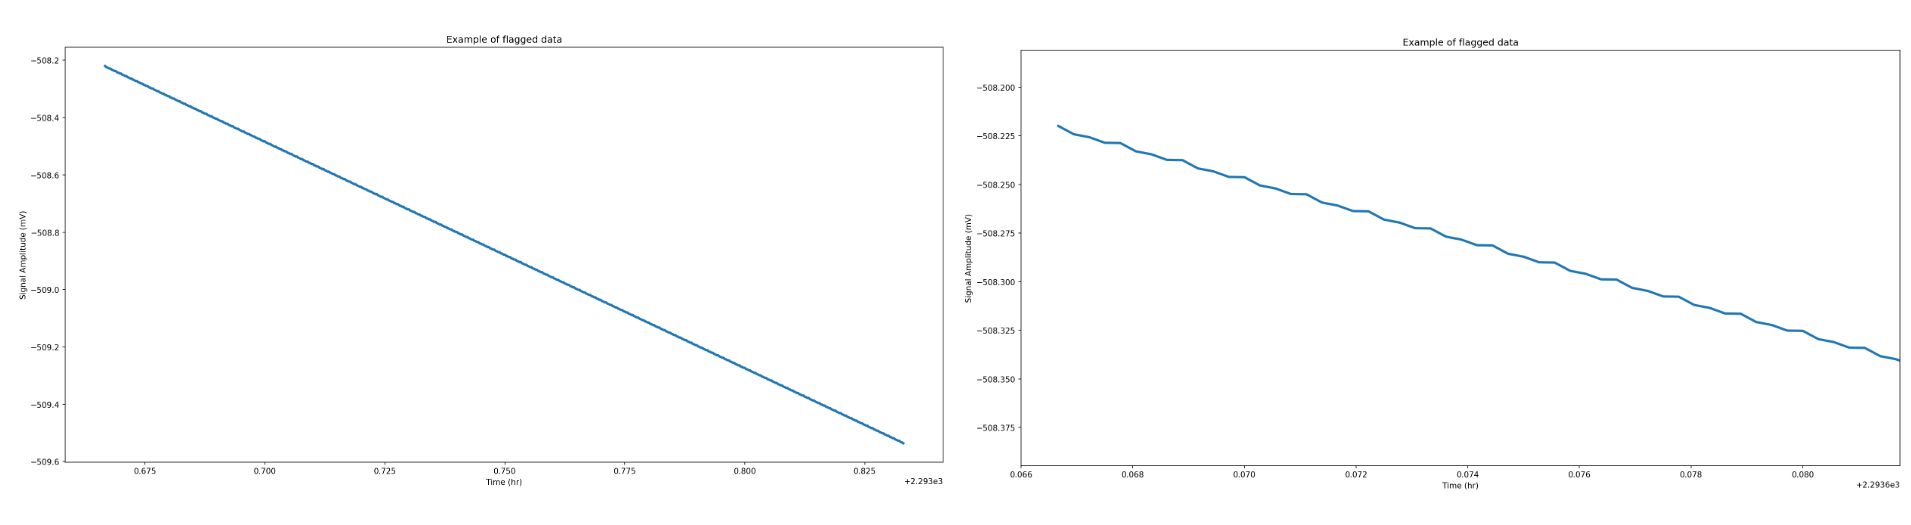
\includegraphics[width=\textwidth]{plan/flagged.png}
\caption{Examples of flagged data: a logger drift segment shown at two zoom levels.}
\label{fig:flagged}
\end{figure}

\section{Data representation: spans, windows and features}
\label{sec:representation}

A central component of the framework is the representation of the time-series data as a collection of fixed-length windows. Given a time-series $T = (x_1, x_2, \ldots, x_n)$, the signal is divided into overlapping or non-overlapping subsequences of length $w$. Each window represents a local segment of the signal at a particular time scale, which allows the analysis to capture both short-term dynamics, such as spikes, and longer-term trends.

Regions of interest that are not of fixed length --- a manually flagged region, a segment returned by a change-point detector, the set of matches to a query --- are represented instead as \emph{spans}: intervals with a start, a duration, and optionally a label. Windows are extracted from spans; the two are not interchangeable, and the distinction is enforced by the type system described in Section~\ref{sec:types}.

To organise the results of analysis, a structured data object referred to as a \emph{Window Matrix} is used. In this representation, each row corresponds to a window, referred by the window's start index, and each column corresponds to a feature extracted from that window. Features include statistical properties (mean, variance), frequency-based features, time-domain characteristics (spike amplitude, width, inter-spike interval), complexity and entropy measures, catch22 canonical features, symbolic encodings, and model outputs such as classification labels and cluster assignments.

The Window Matrix provides a unified structure for storing heterogeneous outputs from multiple analytical techniques, enabling direct comparison and integration. It is important to note what it is not: it carries one row per window and has no alignment to individual timepoints, and so cannot be thresholded to produce regions of interest. That role belongs to the time-aligned \texttt{Scores} profile (Section~\ref{sec:types}).

Figure~\ref{fig:windowmatrix} shows an early example (Chapter~\ref{ch:early}).

\begin{figure}[htbp]
\centering
\figplaceholder{6cm}{Figure 5.2 (T1, bundle): the anatomy of an event. One accepted drop, with its onset, trough,
swing (mV), fall time, recovery time and full width at half maximum marked: the same measures as Chapter~\ref{ch:events}.}
\caption{How an event is measured.}
\label{fig:anatomyevent}
\end{figure}

\begin{figure}[htbp]
\centering
\figplaceholder{5cm}{Figure 5.3 (T1, bundle): the anatomy of a train. Four hours of drops on one channel with each
interval written between onsets; beneath, one line each on what LV and CV2 measure.}
\caption{How a train of events is measured.}
\label{fig:anatomytrain}
\end{figure}

\section{Judging protocol}
\label{sec:judging}

\begin{instructions}
New section, about one page, central to every result. Cover:
\begin{itemize}
  \item the five-word verdict vocabulary;
  \item what ``interesting'' means operationally: in your own words, the rule you applied;
  \item each kind of queue and what it was used for (Table~\ref{tab:queues});
  \item blind presentation, with machine sections masked;
  \item stratified sampling of candidate events by detector agreement and by rare detector family, so that rare
        strata are seen;
  \item carried copies excluded from counts;
  \item your re-test reliability: 98 blind repeats, 94\,\% agreement ($\kappa$ 0.84), 6 changed answers (4 yes to no,
        2 no to yes), so an 11.5\,\% miss per look (95\,\% range 4.6--23\,\%);
  \item your pace: a median of 1.4\,s per verdict;
  \item the limitation: a single labeller, so every precision here is precision against your judgement.
\end{itemize}
\end{instructions}

\begin{table}[htbp]
\caption{Review queues that supply the human judgements in this thesis.}
\label{tab:queues}
\small
\begin{tabularx}{\textwidth}{p{2.2cm} p{4.0cm} r X}
\toprule
\textbf{Queue} & \textbf{Content} & \textbf{Verdicts} & \textbf{Used in}\\
\midrule
Imported labels & 10-minute windows, M2\_aug, early manual labelling & 11,234 & RQ3 baseline forests; reference CNNs\\
3 & Blind random 1/10/30-min windows (M2\_aug, M2\_concat) & 986 & RQ3 blind exam; RQ2 base rate (22\,\%)\\
24 & Spike-seed matches (unblinded) & 61 & RQ2\\
25 & Stratified blind candidate events, M2\_aug & 800 & RQ1; R4 training\\
28 & Stratified blind candidate events, CO, LM, M2\_concat, L\_LM & 1,159 & RQ1; R4 training\\
Library review & Library members & 247 & Accepted set\\
35 & Blind seed panel: drop30, spike37, re-judged dips, random controls & 249 & RQ2 blind test\\
36 & M4 held-out exam, stratified blind candidates & 290 & RQ3 exam, RQ1 on M4\\
\bottomrule
\end{tabularx}
\end{table}

\begin{instructions}
Queues 35 (249 items) and 36 (290) are filled in (5 Nov). Add queue 37 (\emph{S.\ commune}, 263 items) if its exam is
reported. Check the dip-seed queue ids and counts
(256/263 and 94/104) against \src{docs/rq_roundA_2/RQ2b-second-seed.md}.
\end{instructions}

\section{Controls}
\label{sec:controls}

\subsection{Surrogate comparison}

\begin{instructions}
Point back to Section~\ref{sec:surrogates} and say per result chapter which null was used:
\begin{itemize}
  \item paired one-draw phase-randomised runs for the sweep, with 20-draw re-runs prepared;
  \item 200 draws per channel for seed searches;
  \item 200 label shuffles for classifiers;
  \item AAFT for value-reading measures.
\end{itemize}
State the second kind of null, used where humans judge: the blind base rate. 235 of 1,084 random windows were called
interesting (22\,\%), and the blind seed panel's duration-matched random windows give its own controls.
\end{instructions}

\subsection{Cross-channel classification}
\label{sec:crosschannel}

All channels within a recording sit on a single mycelium network with a shared ground, so cross-channel co-occurrence is confounded by construction. A motif family matched across several channels may reflect a recording artefact, a single event propagating through the substrate, or genuine independent recurrence, and these are not the same finding. Matched pairs are therefore classified into three bins by inter-channel lag and waveform correlation (Table~\ref{tab:crosschannel}). A pair counts only if it beats its own random-time null.

\begin{table}[htbp]
\caption[Classification of cross-channel matches]{Classification of cross-channel matches, as implemented in \texttt{Working/cross\_channel.py}. Bin edges are editable in Settings.}
\label{tab:crosschannel}
\begin{center}
\small
\begin{tabular}{p{3.2cm} p{4.6cm} p{5.6cm}}
\toprule
\textbf{Bin} & \textbf{Signature} & \textbf{Interpretation}\\
\midrule
Artifact (common mode) & $|\text{lag}|\le1$\,s and $|r|\ge0.98$ & Recording artefact via the shared ground; flagged for a human, excluded from recurrence counts only once confirmed\\
\addlinespace
Propagation & 1--50\,s lag and $|r|\ge0.5$ & A single network propagation event; counted once\\
\addlinespace
Independent recurrence & Anything else that beats chance & Genuine recurrence; counted once per instance\\
\bottomrule
\end{tabular}
\end{center}
\end{table}

\begin{instructions}
The plan's bins were described qualitatively; give the implemented edges, as in the table. State that only
human-confirmed artefacts are removed. Correction (27 Oct): the ``64 flagged pairs'' were sandbox numbers on g-05; the
real database holds no cross-channel rows. B4's explorer (Chapter~\ref{ch:roundb}) adds a fourth bin, the shared
driver, judges propagation only within a pack, and counts a detector census. Update this table if the census is built
before the freeze.
\end{instructions}

\section{The held-out recording and its exam}
\label{sec:holdout}

The thesis plan, dated 14 August 2026, held one recording out: M4, a 16-channel oyster recording of 505 hours. It was not to be inspected, labelled, clustered or used for any parameter selection. It was reserved for a single end-to-end run after the analysis was frozen. The plan put it this way: ``A holdout declared in advance is a matter of record; a holdout declared afterwards is a claim.'' This section reports, in the same spirit, how far that record held.

\begin{table}[htbp]
\caption{Exposure record of the held-out recording M4 (times AEST). From \texttt{audit\_log}, \texttt{runs} and \texttt{annotations}.}
\label{tab:exposure}
\small
\begin{tabularx}{\textwidth}{p{3.3cm} X}
\toprule
\textbf{When} & \textbf{What}\\
\midrule
4 Aug 2026 & 11 early runs, and one ``interesting'' annotation on channel 0 (samples 748,871--763,617), made before the plan declared M4 held out\\
14 Aug & Thesis plan declares M4 held out\\
Early Oct & Held-out lock enforced: every route refuses M4\\
17 Oct, 15:02 & Lock switched off for the demonstrations (audit 519)\\
19 Oct & Detector sweep: 1,264 runs on M4 (632 surrogates), with settings chosen on other recordings; imported into Discovery\\
20--21 Oct & M4's detection rates visible on the Discovery Map and in the poster's detector figure (marked held out)\\
26 Oct, 08:34 & Lock switched on again (audit 536)\\
26 Oct, 08:40 & Exam manifest frozen, sha256 \texttt{db32fdc7\ldots} (audit 537)\\
26 Oct, 08:52 & Stratified blind sample drawn: queue 36, 290 candidate events (audit 538)\\
26 Oct, 09:11 & Manifest amendment 1, adding the CNNs, before any judging (audit 539)\\
{[date]} & Exam judged with the lock briefly off [audits], then scored once\\
\bottomrule
\end{tabularx}
\end{table}

\begin{instructions}
In your words, state what the exposure was and was not:
\begin{itemize}
  \item what M4 was exposed to: detector output, displayed;
  \item what it was never exposed to: no human verdict on any M4 detection, no Library entry, no model trained or tuned
        on it, and no detector parameter chosen on it.
\end{itemize}
Then describe the exam as run:
\begin{itemize}
  \item the manifest: model and file hashes, the sampling design, the metrics, and the protocol;
  \item the sample: 5 agreement strata of 40, plus 6 rare-detector strata of 15, from 832,136 candidate events (built
        from 1,186,189 detections);
  \item blind judging;
  \item the scorer's refusals, which make the exam one-shot (\src{scripts/m4_exam_score.py}).
\end{itemize}
Manifest: \src{docs/rq_roundA_2/exam/M4-exam-manifest.json}. Amendment:
\src{docs/rq_roundA_2/exam/M4-exam-amendment-1.json} (sha256 \texttt{5286bac3\ldots}).
\end{instructions}

\section{Evaluation criteria}
\label{sec:evaluation}

Two distinct things are evaluated in this thesis and they should not be conflated.

The \textbf{analysis methods} are evaluated on four things:
\begin{itemize}
  \item their precision against blind human judgement;
  \item their output against a matched surrogate of the same signal;
  \item their transfer to recordings they were not developed on;
  \item their robustness to the baseline wander and noise characteristic of these recordings.
\end{itemize}
Where possible, results are compared with the performance of the methods described in Chapter~\ref{ch:litreview}.

The \textbf{instrument} is evaluated on generalisation, by the held-out exam, and on two tested assertions. A recipe rerun gives the same output, and no machine-derived label enters the human label store (Section~\ref{sec:tooleval}).

\section{Ethics and risk}
\label{sec:ethics}

This project involves the analysis of previously recorded experimental data and does not involve or harm human or animal subjects. No ethics approval was required.

Data handling follows appropriate practices to ensure integrity and reproducibility, as per the Privacy Act of 1988 \cite{privacyact}. All analysis code is documented and, where possible, made publicly available to support transparency. All data and code used from outside sources is responsibly sourced from open-source and publicly available repositories.

Two project risks were recorded in the plan. The first was computational: all-pairs similarity search over multi-hundred-hour recordings exceeds what is practical on a single workstation. This was mitigated by seeded search and by running long jobs on UQ's rangpur cluster. The second was that the signals might not show clear or consistent recurring patterns. Because every result is reported against a null, a finding of no recurrence would have been reportable rather than a failed project.

\begin{instructions}
Add the risk that did materialise: data loss. On 21 Sep, \texttt{git worktree remove} followed a directory junction
and emptied the real \texttt{DATA/db} and \texttt{DATA/derived} (7.8\,GB). The database was recovered from a sandbox
copy and the channels were re-derived. The mitigations that followed: the bridge's sandbox copies, automatic backups at
start-up, and the rule to unlink junctions first. Also note the public dataset's licence: Adamatzky's four-species data
is CC BY 4.0.
\end{instructions}
